\chapter{Models, Consistency and Processes
    \pgsize{15 p.}
}
\label{chap:networks}

\mnote{Chapter summary}
In this chapter, we discuss general terms and notions to clarify the scope of this thesis.
We discuss different dimension of consistency, its specification and consistency preservation, as well as the process of specifying consistency with a depiction of the involved roles and relevant scenarios.
We introduce the general notion of models used in this thesis and the notations that we use for them.
Finally, we introduce a running example.


%%
%% CONSISTENCY NOTIONS
%%
\section{Dimensions of Consistency, Specification and Preservation}

\mnote{Consistency overview}
In the following, we clarify different dimensions of how consistency can be considered and specified, which types of consistency can be distinguished and how these types induce different processes of checking and enforcing them.
This leads to the restriction of our work to normative specifications of preservation for structural consistency relations.

\subsection{Normative and Descriptive Specification}
\label{chap:networks:notions:normative_descriptive}

\mnote{Specification types}
We have yet informally considered consistency as the absence of some kind of contradictions in different models.
It is, however, unclear when to consider information in models contradictory.
Consistency can be considered \emph{normatively} or \emph{descriptively}, depending on whether a notion of consistency already exists.

\mnote{Normative consistency}
With a normative (or \emph{prescriptive}) specification of consistency, we consider models consistent whenever we want them to be consistent.
Thus, if someone specifies consistency, for example, in terms of a transformation, models are considered consistent when they adhere to that specification.
No matter what this person defines as consistent is actually considered as consistent, i.e., the transformation \emph{prescribes} consistency.
Such a specification can always be considered \emph{correct}, because there is no external specification to which it has to adhere.
For example, it is usually not predefined when an architecture specification, be it in \gls{UML}, \gls{PCM}, or some other language, is considered consistent to its realization in code, so a transformation normatively defines how consistency is considered.

\mnote{Descriptive consistency}
Following a descriptive specification of consistency, we assume that consistency is already defined and we have to adhere to that definition.
Thus, if somebody specifies a transformation, it has to following that existing definition of consistency. 
The transformation does only \emph{describe} consistency.
Such an existing specification may not exist explicitly, but can exist implicitly, for example, because there is some common notion of consistency for specific languages.
A descriptive specification may be \emph{incorrect}, because it has to adhere to the existing definition of consistency.
For example, there is, at least for most constructs, a common understanding of when \gls{UML} class models and Java code are considered consistent, even if this understanding is not represented explicitly.
Thus, any transformation has to describe that existing notion of consistency.

\mnote{Normative specification in thesis}
In this thesis, we always assume a normative specification of consistency.
This does not mean that we exclude languages for which some notion of consistency already exists, such as \gls{UML} and Java code, but we assume that a specification of that consistency is normative.
This means, if there is an existing notion of consistency, we do not consider whether the specification is correct with respect to that existing notion, but we assume it to be correct by construction.
It is subject to other research, including general requirements engineering and especially transformation validation~\cite{rahim2015SurveyTransformationVerification-SoSym}, to check whether a transformation is correct with respect to some expectation, reflecting an existing notion of consistency.
This includes validation or verification of invariants~\cite{cabot2010VerificationInvariants-JSS} or contracts~\cite{azizi2017ContractVerification-ICCKE, vallecillo2012FormalTesting-FMMDE}.


\subsection{Structural and Behavioral Consistency}
\label{chap:networks:notions:types}

\mnote{Execution semantics as distinction}
In addition to the distinction between normative and descriptive consistency, we can distinguish different types of consistency relations.
From a pragmatic perspective, we can at least differentiate between \emph{structural} and \emph{behavioral} consistency relations.
While structural consistency concerns everything that has no execution semantics, behavioral consistency concerns semantics and thus also, for example, method bodies.
Structural consistency can thus be checked without executing the model, comparable to the distinction between \emph{static} and \emph{execution} semantics of models, as introduced in \autoref{chap:foundations:modeling:models}.
For example, having the same classes and method signatures in a \gls{UML} model and Java code would be considered a structural relation, whereas the equivalence of a \gls{UML} state machine and its Java code implementation would be considered a behavioral relation, because they need to have the same execution semantics.
Thus, the mechanisms for checking these different types of consistency are supposed to be different.

\mnote{No strict separation}
The distinction between structural and behavioral relations is, however, not strict.
If, for whatever reasons, two Java code artifacts shall be kept consistent, although they share a behavioral relation it can reduce to a structural relation when exactly the same elements have to be contained.
In consequence, one might argue that structural consistency relations are a special case of behavioral relations, for which we do not need to consider the execution semantics of the model but only its static structure.

\mnote{Decidability as distinction}
From a theoretical perspective, we can distinguish between decidable consistency and undecidable consistency relations.
While structural consistency relations do not consider execution semantics and are thus decidable, behavioral consistency relations will usually be undecidable, because as soon as we have Turing-complete descriptions of behavior, we cannot decide their semantic equivalence. %\todo{add cite?}
An approach that checks behavioral consistency can be further distinguished regarding the statements he is able to make regarding consistency relations:
\begin{properdescription}
    \item[Universally quantified:] The approach can validate that a consistency relation holds for all instances of the modeled system. This can, for example, be achieved with verification techniques, model checking and other analyses. An exemplary application scenario is the equivalence of decidable behavior descriptions.
    \item[Existentially quantified:] The approach can validate that a consistency relation holds at least for some instances of the modeled system. This can, for example, be achieved with tests. In the best case, the test cases cover a representative subset of the possible instances. An exemplary application scenario is the equivalence of undecidable behavior descriptions.
    \item[Statistical:] The approach can make statistical statements about the consistency relations, such as the probability for a relation to be fulfilled in an instance. This can, for example, be achieved by simulation. An exemplary application is consistency between quality requirements and the system realization, such as the fulfillment of a performance requirement in the implementation.
\end{properdescription}
While universally quantified statements can only be made about decidable consistency relations, existentially quantified and statistical statements can be made about both decidable and undecidable consistency relations, although preferably used for undecidable relations.

\mnote{Structural relations supposed to be decomposable}
At a Dagstuhl seminar regarding multidirectional transformation~\cite{cleve2019dagstuhl} different consistency relation scenarios were considered, in which more than two models were related.
A central insight was that probably relations between more than two models can be decomposed into binary relations as long as the relations are structural.
Whether two or more models fulfill a behavioral requirement, however, may not easily decomposed into multiple binary relations between model pairs.

\mnote{Structural relations in thesis}
In this thesis, we focus on structural relations.
This does not mean that our contributions are restricted to these kinds of structural relations.
In fact, we do not make assumptions that exclude other types of consistency relations, so as long as they conform to the formalism that we propose, our contributions also apply for them.
We do, however, only consider structural relations in our examples, considerations and evaluations, such that generalization to other relations types needs to be evaluated.


\subsection{Checking and Preserving Consistency}

\mnote{Checking and preserving consistency}
Based on a specification of consistency and potentially its preservation, consistency between different models can be checked and potentially enforced during the development of a system.
Basically, we can distinguish whether a process is only \emph{checking} or also \emph{preserving} consistency.
Some consistency relations may only be checked and have to be manually ensured, whereas others can (semi-)automatically be enforced.

\mnote{Enforcing structural and checking behavioral relations}
Behavioral consistency relations are usually hard to enforce but can, in the best case, only be checked.
This also includes relations that define quality properties of behavior, such as performance of a behavior specification regarding performance requirements.
On the contrary, structural consistency relations can often also be enforced, at least collecting some additional information from the developer.

\mnote{Efficiency and granularity of checking and enforcing relation types}
In addition, structural consistency relations can and should be checked and enforced more often, because they can be checked in a rather fine-grained way and more efficiently, in the extreme case even just-in-time.
Checking behavioral relations may also include long-running analyses or simulations and may only make sense to be checked at specific points in time, indicated by the developer.
This at least applies to relations for which only existentially quantified or statistical statements can be made.
For example, adding a an architectural component to a \gls{PCM} model can and should directly lead to the creation of an implementing class in java code. %$ or method in \gls{UML} can and should directly lead to the creation of an appropriate class or method in Java.
%Adding an architectural component can directly lead to the creation of an implementing class.
But whether a Java method fulfills some behavioral consistency relation to another model, such as the behavioral service specifications in a \gls{PCM} model, usually makes sense less often, as it requires more coarse-grained modifications to achieve consistency and checking may take more time because of complex analyses or simulations to run.
The developer may explicitly indicate when a development state is reached at which behavioral consistency relations can be checked.
For behavioral relations about which universally quantified statements can be made, such as a security analysis, it may be up to the scenario whether checks should be performed just-in-time or only at specific points in time.

\begin{figure}
    \centering
    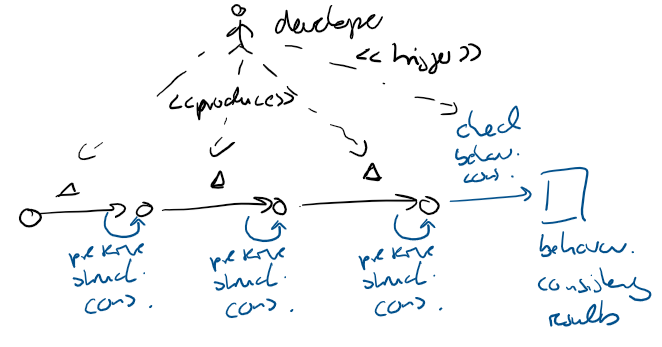
\includegraphics[width=0.8\textwidth]{figures/prologue/networks/process_structure_behavior.png}
    \caption[Process for preserving structural and behavioral consistency]{Proposed process for continuously preserving structural and explicitly checking behavioral consistency}
    \label{fig:networks:process_structure_behavior}
\end{figure}

\mnote{Fine-grained preservation of structural relations}
In consequence, the distinction between structural and behavioral consistency relations is also relevant for the processes of checking and preserving consistency.
While structural consistency relations may be preserved often in a fine-grained way, behavioral consistency relations may be checked less often.
We depict the proposed process in \autoref{fig:networks:process_structure_behavior}.
In the best case, a consistency mechanism can give hints to potential behavioral consistency violations more often.
For example, a performance-relevant modification of the implementation could lead to a hint for the developer that performance may be affected by his modification with the information about the previous analysis result, such that he or she can guess whether his modification will violate the requirement.
Given the information that a response time requirement of 10 milliseconds was fulfilled during the last check by an actual response time of 1 millisecond could help the developer to decide that his modification will not violate that requirement.

\mnote{We focus on structural relations}
In this thesis, we are interested in processes that continuously preserve and not only check consistency.
This is why we explicitly focus on structural consistency relations in this thesis, although the insights might be transferable to behavioral relations as well.
As another consequence, those structural relations that we consider are supposed to be decomposable into binary relations, as discussed in \autoref{chap:networks:notions:types}.



%%
%% CONSISTENCY SPECIFICATION PROCESS
%%
\section{Consistency Specification Process}
\label{chap:networks:specification_process}

\begin{figure}
    \centering
    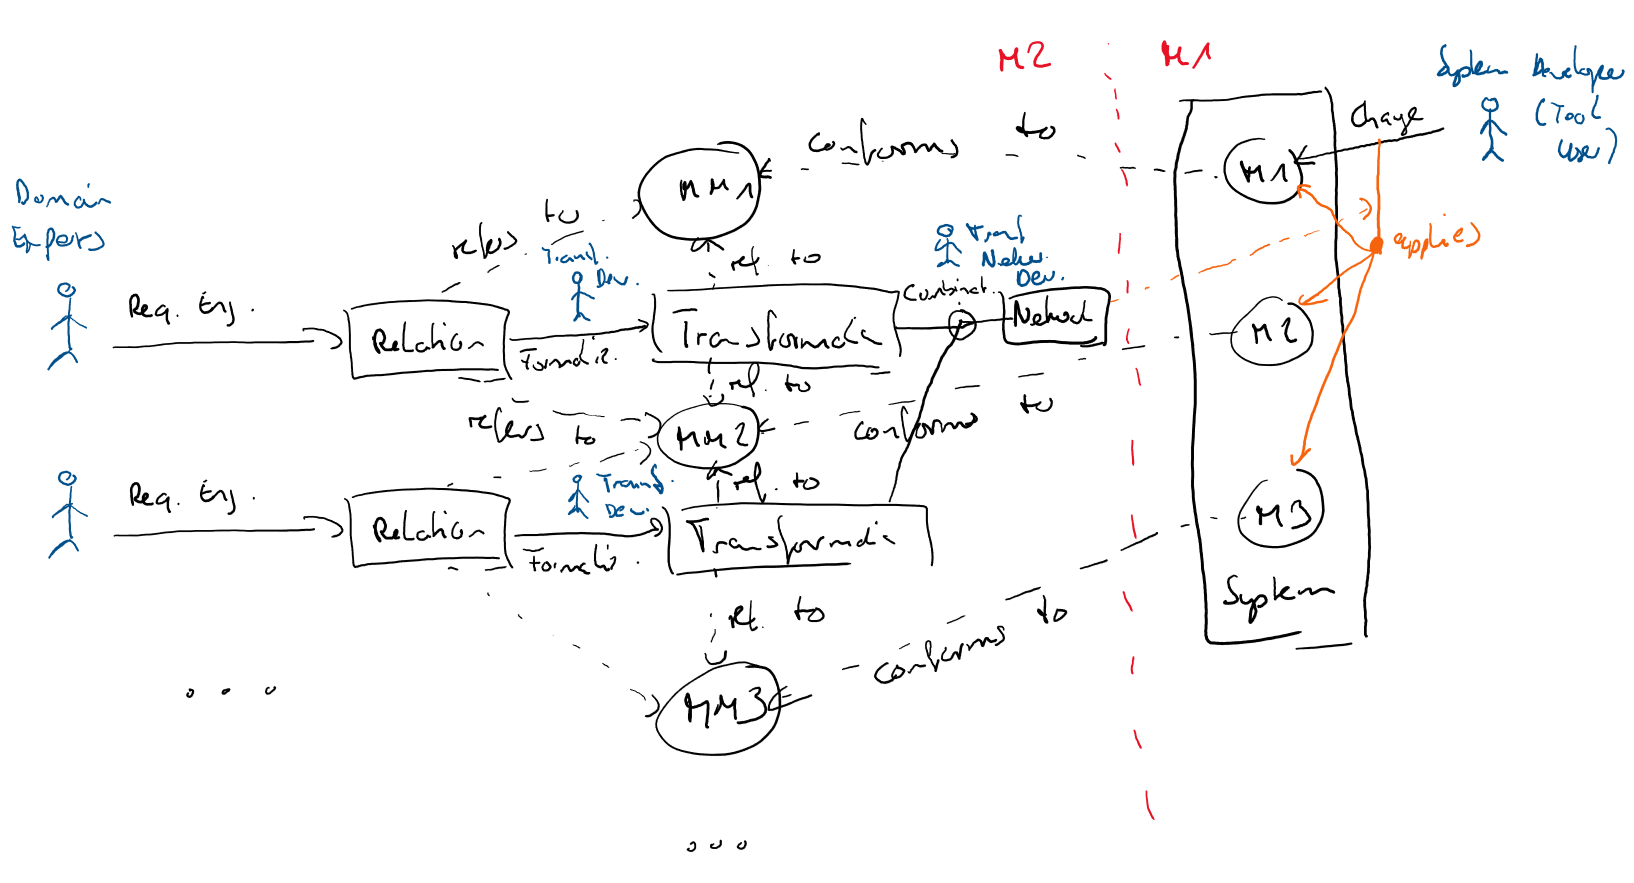
\includegraphics[width=\textwidth]{figures/prologue/networks/roles_and_process}
    \caption[Roles in a transformation network specification process]{Roles involved in a process for specifying a transformation network, their responsibilities and dependencies. Extended from~\owncite{klare2019dagstuhl}.}
    \label{fig:networks:roles_and_process}
\end{figure}

\mnote{Roles and scenarios}
In this thesis, we are concerned with the process of specifying consistency in terms of a transformation network and different problems arising in that process.
We therefore discuss which roles are involved in that process and which different scenarios can be considered that induce requirements and exemplify the application contexts of our later contributions.
\autoref{fig:networks:roles_and_process} gives an overview of the roles and the essential specification process.
While that specification process is concerned with the metamodel level (M2), a transformation network is finally applied at the model level (M1) to a concrete system under development.

\subsection{Roles}

\mnote{Roles in the consistency process}
The specification of a transformation network involves the definition of the individual transformations by \emph{domain experts} and \emph{transformation developers} as well as their combination to a network by \emph{transformation network developers}.
The usage of the network, on the other hand, involves its application to changes to a system under development by a \emph{system developer}, sometimes also called \emph{tool user}~\cite{klare2019dagstuhl}.
Apart from the explicit transformation network, these roles and their responsibilities are comparable to the ones that were defined in a working group of a Dagstuhl seminar, in which the author of this thesis participated~\cite{klare2019dagstuhl}.

\mnote{Roles for the specification}
A domain expert has the knowledge about the consistency relations between two (or more) tools and their languages or, more specifically, the metamodels describing them.
He performs the requirements engineering task for the information to define in a transformation.
A transformation developer is then responsible for formalizing these relations and their preservation in a transformation.
We will usually only refer to the transformation developer, as for us it is not of specific interest where the information about the relations comes from but only that it is encoded into a transformation.
Finally, a transformation network developer combines different transformations, which were usually developed by different transformation developers, to a transformation network.
It may even be possible that several transformation network developers compose several transformation networks to a larger transformation network. 
Whenever the distinction is not relevant, we will refer to both transformation and transformation network developers simply as \emph{transformation developers}.

\mnote{Roles for the usage}
Concrete systems are developed with the use of transformation networks by system developers, who perform changes of models via the tools they use.
Thus, we also call them tool users.
Usually different system developers will be responsible for different models.
In our introductory example, we distinguished between software architects, developers, requirements engineers and so on.
Performing changes leads to the application of the transformation network to restore consistency of the models.
In this thesis, we refer to system developers as \emph{users}, as they are the ones using the transformation networks we are concerned with.

\mnote{Multiple roles fulfillable by same persons}
The roles reflect the different responsibilities when specifying and using transformation networks.
Several of them can, however, be fulfilled by the same persons.
This especially applies to domain experts and transformation developers.
The same person may know about the relations as a domain expert and formalize them in a transformation.
Potentially, a domain expert may even be the one who develops a concrete system as a system developer.


\subsection{Scenarios}

\mnote{Generic and project-specific transformations}
Both for the development of transformations as well as for the combination of transformations to a network, different development scenarios can be distinguished.
Transformations can be developed generically or specific for a project.
\begin{properdescription}
    \item[Generic:] Transformations are developed as artifacts off-the-shelf, which can be used in any project. This especially applies for descriptive transformations (cf. \autoref{chap:networks:notions:normative_descriptive}), which encode a common understanding of consistency, such as for \gls{UML} class models and Java code.
    \item[Project-specific:] Transformations are developed specific for a project. This can occur when a project requires specific rules how elements shall be related. For example, the mapping of components to their realization in the implementation can be specific to the project~\cite{langhammer2017a}. Project-specific transformations can, eventually, later be used in a generic way.
\end{properdescription}

\mnote{Big bang and continuous combination}
The combination of transformations to networks can be distinguished especially regarding the point in time at which the combination takes place.
\begin{properdescription}
    \item[Big bang:] Transformations are developed first and after they have been completed, a transformation network developer combines them to a network. Problems regarding the compatibility of the transformations are first recognized during this combination, thus transformations may need to be adapted afterwards to properly work together.
    \item[Continuous:] Transformations are combined to a network already during their development. Starting with partial or even empty transformations, the structure of the network can be defined early. This allows for a continuous validation of compatibility of the developed transformations. Ultimately, even an online checking of compatibility after each change to a transformation can be performed to get early feedback.
\end{properdescription}

\mnote{Effects of combination process}
For us, it is not relevant whether transformations are developed in a generic or project-specific way.
The distinction of scenarios in which transformation networks are developed is, however, of special interest.
It can be beneficial for transformation developers to get feedback on the compatibility of their developed transformations with others on-the-fly.
This makes locating a problem easier, because only the last changes may have introduced it, whereas with an a-posteriori checking in a big bang process the effort to find compatibility problems may increase because of missing locality.

\mnote{Mixing processes}
While both generic as well as project-specific transformations can be mixed in a single project, also the process of combining them may be mixed.
Some of the transformations may be integrated in a big bang fashion, whereas others are continuously integrated.
This can also be a result of where the transformations come from.
A generic transformation cannot be continuously integrated, because it is not specific for a single project to integrate it into.


%%
%% MODELS AND METAMODELS
%%
\section{Models and Metamodels}
\label{chap:networks:models}

\begin{table}
    \centering
    \small
    \renewcommand{\arraystretch}{1.4}%
    \rowcolors{1}{\secondlinecolor}{\firstlinecolor}
    \begin{tabular}{R{4.8cm} L{5cm}}
        \toprule
        \rowcolor{\headinglinecolor}
        \multicolumn{2}{c}{\textbf{Properties and Classes}}\\
        $P$
            & Property (attribute or reference) \\
        $\instances{P} = \setted{p_1, p_2, \dots}$     
            & Property values of a property $P$ \\
        $\class{C}{} = \tupled{P_1, \dots, P_n}$
            & Class \\
        $\instances{\class{C}{}} = \setted{\object{o}{} = \tupled{p_1, \dots, p_n} \mid p_i \in \instances{P_i}}$ 
            & Instances (objects) of a class $\class{C}{}$\\
        $\object{o}{} \in \instances{\class{C}{}}$
            & Object of a class $\class{C}{}$ \\
        \midrule
        \rowcolor{\headinglinecolor}
        \multicolumn{2}{c}{\textbf{(Meta-)Models}}\\
        $\metamodel{M}{} = \setted{\class{C}{1}, \dots, \class{C}{m}}$
            & Metamodel\\
        $\metamodelinstanceset{M}{} = \setted{\model{m}{} \mid \model{m}{} \subseteq \bigcup_{\class{C}{} \in \metamodel{M}{}} \instances{\class{C}{}}}$
            & Instances of a metamodel\\
        % $\metamodelset{M} = \setted{\metamodel{M}{1}, \dots, \metamodel{M}{k}}$
        %     & Set of metamodels\\
        % $\metamodelsetinstanceset{M} = \setted{ \setted{\model{m}{1}, \dots, \model{m}{k}} \mid \model{m}{i} \in \metamodelinstanceset{M}{i}}$
        %     & Instances of a metamodel set $\metamodelset{M}$\\
        $\metamodeltuple{M} = \tupled{\metamodel{M}{1}, \dots, \metamodel{M}{k}}$
            & Tuple of metamodels\\
        $\metamodeltupleinstanceset{M} = \metamodelinstanceset{M}{1} \times \dots \times \metamodelinstanceset{M}{k} = \setted{ \tupled{\model{m}{1}, \dots, \model{m}{k}} \mid \model{m}{i} \in \metamodelinstanceset{M}{i}}$
            & Instances of a metamodel tuple $\metamodeltuple{M} = \tupled{\metamodel{M}{1}, \dots, \metamodel{M}{k}}$\\
        $\model{m}{} \in \metamodelinstanceset{M}{}$
            & Model of metamodel $\metamodel{M}{}$\\
        $\modeltuple{m} \in \metamodeltupleinstanceset{M}$
            & Model tuple of a metamodel tuple $\metamodeltuple{M}$\\
        \bottomrule
    \end{tabular}
    \caption[Models, metamodels, their elements and notations]{Models, metamodels, their elements and notations}
    \label{tab:networks:elements}
\end{table}

\mnote{Notation overview}
The most essential elements used for descriptions in this thesis are models and the metamodels describing them.
We have already introduced in \autoref{chap:foundations} what we consider a model and that we adhere to the modeling formalism defined by the \gls{MOF}.
We use a sufficiently simplified notion of models, metamodels, and their elements, for which we give an overview in \autoref{tab:networks:elements}.
In the following, we introduce the used notation and its conventions, as well as the elements used for modeling.
Finally, we clarify assumptions that we make and discuss their impact.


\subsection{Notation and Conventions}

\mnote{Modeling levels}
In general, we use variables of uppercase letters for all elements at the metamodel level (M2), such as $\metamodel{M}{}$ for a metamodel or $\class{C}{}$ for a class, whereas we use lowercase letters for all elements at the model level (M1), such as $\model{m}{}$ for a model and $\object{o}{}$ for an object.

\mnote{Notation for model and metamodel level relations}
We use the notations for sets and tuples introduced in \autoref{chap:foundations:notations} for denoting sets and tuples of the different elements, such as metamodels and models.
When considering multiple metamodels or models, we are usually not interested in their order and usually the same model or metamodel cannot appear twice.
Still, we always treat them as tuples rather than sets to be able to easily relate a model to its metamodel by its index within the tuple.
Thus, if not further specified, we use the same indices to relate element at the metamodel and the model level, such as as $\model{m}{1}$ being an instance of $\metamodel{M}{1}$, i.e., $\model{m}{1} \in \metamodelinstanceset{M}{1}$.
This could also be expressed by an explicit instantiation relation, but the used notation is more concise and thus proposes to easy readability.


\subsection{Modeling Elements}

\mnote{Elements overview}
In general, we consider metamodels as a composition of \metaclasses, which, in turn, are composed of properties representing attributes or references.
Models instantiate metamodels and are composed of objects, which are instances of \metaclasses and, in turn, consist of property values, which instantiate properties.

\mnote{Properties and property values}
We denote \emph{properties}, which are the information a \metaclass consists of, such as attributes or references, as $P$ and the \emph{property values} as instances of a property as $\instances{P} = \setted{p_1, p_2, \dots}$ of property $P$. 
We do not need to further differentiate different types of properties into attributes and references, like it is done in other formalizations, such as the \gls{OCL} standard~\cite[A.1]{ocl} or the thesis of \citeauthor{kramer2017a}~\cite[2.3.2]{kramer2017a}.

\mnote{Classes and objects}
We denote \emph{meta-classes}, in the following shortly called \emph{classes}, as tuples of properties $\class{C}{} = \tupled{P_1, \dots, P_n}$. 
Instances of a class are \emph{objects}, each being a tuple of instances of the properties of the class.
We denote all instances of a class $\class{C}{}$ as $\instances{\class{C}{}} = \setted{\object{o}{} = \tupled{p_1, \dots, p_n} \mid p_i \in \instances{P_i}}$.

\mnote{Metamodels and models}
We denote a metamodel $\metamodel{M}{} = \setted{\class{C}{1}, \dots, \class{C}{m}}$ as a finite set of classes.
The instances of a metamodel are sets of objects $\metamodelinstanceset{M}{} = \setted{\model{m}{} \mid \model{m}{} \subseteq \bigcup_{\class{C}{} \in \metamodel{M}{}} \instances{\class{C}{}}}$.
In other work like~\cite{stevens2020BidirectionalTransformationLarge-SoSym}, such instance sets are also called \emph{model sets} and implicitly define a metamodel, thus representing a lightweight definition of metamodels by simply enumerating its instances.
Each instance of a metamodel is called a \emph{model}, and represents a finite set of objects that instantiate the classes in the metamodel.
For a tuple of metamodels $\metamodeltuple{M} = \tupled{\metamodel{M}{1}, \dots, \metamodel{M}{k}}$, we denote the set that contains all sets of instances of that metamodels as $\metamodeltupleinstanceset{M} = \setted{ \tupled{\model{m}{1}, \dots, \model{m}{k}} \mid \model{m}{i} \in \metamodelinstanceset{M}{i}}$.

\mnote{Valid models}
With $\instances{\class{C}{}}$ and $\metamodelinstanceset{M}{}$, we denote the sets of instances of a class and metamodels, i.e., the objects and models instantiating them.
Usually, additional constraints exist that further restrict these sets.
For example, a property can represent a reference to another object, thus if a class contains a specific property value representing a reference to an object, the referenced object must be contained in the model as well.
Thus, the sets of \emph{valid} instances of classes and metamodels are usually only subsets of the sets we denote with $\instances{\class{C}{}}$ and $\metamodelinstanceset{M}{}$, respectively.
For reasons of simplicity, we will, however, usually only refer to the denoted instance sets.
The statements still apply to the sets of valid object and models as subsets of considered sets.

%\todo{Ergänzen, dass wir die Fälle diskutieren, wo sich das nicht übertragen lässt (konkrete Kompatibilität). Dort dann erklären, wie Kombination aus Restriktion auf valide Modelle + Konsistenzrelationen nur gewünsche Modellmengen zulässt. Außerdem diskutieren, warum Kompatibilität nicht auf validen Modellen definiert ist.}

%\todo{Discuss valid models, why we do not consider them and prove that invariants + consistency relations can express any consistency relation.
%A single relation can consider constraints on the single models, but combination (even within one transformation) can easily contradict constraints of a model.
%New:
%Discuss valid models here and why we do not further consider them. Discuss at end of (or somewhere in) compatibility how combination of valid model restriction and consistency relations can express any restriction to desired model sets.}

%\todo{Idee für das Ausschluss-Problem (Für Student darf kein Employee existieren): Entweder darf nie ein entsprechender Employee existieren, dann müssen die Modelle allesamt ausgeschlossen werden (valid models). Wenn es in bestimmten Modellen auftreten darf, muss der Kontext einer Konsistenzrelation richtig festgelegt sein, damit sie abbildet unter welchen Bedingungen der Employee existieren darf. Geht aber nicht, weil Employee einfach in keiner Relation auftauchen könnte (man will nie, dass ein Employee für ein anderes Element vorhanden ist), aber man will, dass er in bestimmten Situationen nicht auftauchen darf.}



\subsection{Assumptions}
\label{chap:networks:models:assumption}

\mnote{Finite models}
We assume models to be finite, so for each model $\model{m}{}$, we assume that $|\model{m}{}| < \infty$.
Additionally, our proposed formalism assumes objects to be unique within a model $\model{m}{}$. 
This is already implicitly covered by the definition of $\metamodelinstanceset{M}{}$ for the instances of a metamodel $\metamodel{M}{}$. 

\mnote{Unique elements}
In practice, it is usually allowed to have the same object, i.e., an element with the same type, attribute and reference values, multiple times within the same model. 
This is, however, only a matter of identity, which, in practice, is given at least by different objects being placed at specific places in memory.
We assume, without loss of generality, the necessary information to distinguish two elements to be represented within properties of these elements.

% Our definition of models does not restrict validity of models apart from being a collection of instances of the classes in the metamodel.
% It is possible to define further constraints for metamodels that restrict their valid instances.
% We intentionally do not consider such restrictions of valid models, because even a single transformation 



%%
%% RUNNING EXAMPLE
%%
\section{Running Example}
\label{chap:networks:example}

%\todo{Address von Resident in "Location" auslagern und Address von "Person" in Address auslagern. Also remove $R'_{ER}$ and move it to compatibility chapter, as it is not yet relevant here.}

\begin{figure}
    \centering
    %% From motivational_example in MPM4CPS paper

\newcommand{\hdistance}{14em}
\newcommand{\classwidth}{6em}

\begin{tikzpicture}

% Person
\umlclassvarwidth{person}{}{Person\sameheight}{
firstname\\
lastname\\
address\\
income
}{\classwidth}

% Employee
\umlclassvarwidth[,above right=2em and \hdistance of person.east, anchor=south]{employee}{}{Employee\sameheight}{
name\\
socsecnumber\\
salary
}{\classwidth}

\umlclassvarwidth[,below=4em of employee.south, anchor=north]{resident}{}{Resident\sameheight}{
name\\
address\\
socsecnumber
}{\classwidth}


% CONSISTENCY RELATIONS
\draw[consistency relation] (person.north) |- node[pos=0, above left] {$p$} node[pos=0.75, above] {$\consistencyrelation{CR}{PE}$} node[pos=1, above left] {$e$} (employee.west);
\draw[consistency relation] (employee.south) -- node[pos=0, below left] {$e$} node[right, align=left] {$\consistencyrelation{CR}{ER}$}% /\\ $R'_{ER}$} 
node[pos=1, above left] {$r$} (resident.north);
\draw[consistency relation] (resident.west) -| node[pos=0, below left] {$r$} node[pos=0.25, below] {$\consistencyrelation{CR}{PR}$} node[pos=1, below left] {$p$} (person.south);

\draw[consistency relation 2] (person.east) -- node[pos=0, below right] {$p$} ++(0.35*\hdistance,0) -- node[pos=0, above=0.5em] {$\consistencyrelation{CR}{PER}$} node[pos=1, above left] {$e$} ([yshift=1em]employee.south west);
\draw[consistency relation 2, -latex] ([xshift=0.35*\hdistance]person.east) -- node[pos=1, below left] {$r$} ([yshift=-1em]resident.north west);

\node[consistency related element 2, below left=5em and 2em of person.south west, anchor=north west, inner sep=0em] (relations1) {
$\begin{aligned}
    \consistencyrelation{CR}{PER} =\; &
            \setted{\tupled{p,e,r} \mid 
            %& 
            \mathvariable{p.firstname} + \text{\enquote{\textvisiblespace}} + \mathvariable{p.lastname} = \mathvariable{e.name} = \mathvariable{r.name} \\
            &
            \land \mathvariable{p.address} = \mathvariable{r.address}
            \land \mathvariable{p.income} = \mathvariable{e.salary} \\
            &
            \land \mathvariable{e.socsecnumber} = \mathvariable{r.socsecnumber}
        }
\end{aligned}$
};

\node[consistency related element, below=0.5em of relations1.south west, anchor=north west, inner sep=0em] {
$\begin{aligned}
    \consistencyrelation{CR}{PE} =\; &
            \setted{\tupled{p,e} \mid %\\
            %& 
            \mathvariable{p.firstname} + \text{\enquote{\textvisiblespace}} + \mathvariable{p.lastname} = \mathvariable{e.name}%\\
            %& 
            \land \mathvariable{p.income} = \mathvariable{e.salary}
        }\\[0.3em]
        \consistencyrelation{CR}{PR} =\; &
            \setted{\tupled{p,r} \mid %\\
            %& 
            \mathvariable{p.firstname} + \text{\enquote{\textvisiblespace}} + \mathvariable{p.lastname} = \mathvariable{r.name}%\\
            %& 
            \land \mathvariable{p.address} = \mathvariable{r.address}
        }\\[0.3em]
        \consistencyrelation{CR}{ER} =\; &
            \setted{\tupled{e,r} \mid %\\
            %& 
            \mathvariable{e.name} = \mathvariable{r.name} %\\
            %& 
            \land \mathvariable{e.socsecnumber} = \mathvariable{r.socsecnumber}
        }%\\
    % R'_{ER} =\; &
    %         \setted{\tupled{e,r} \mid %\\
    %         %& 
    %         e.name.toLower = r.name\\
    %         & \land e.socsecnumber = r.socsecnumber
    %     }
\end{aligned}$
};

\end{tikzpicture}
    \caption[Three metamodels with exemplary consistency relations]{Three simple metamodels for persons, employees and residents. One ternary relation $\consistencyrelation{CR}{PRE}$ between them and three binary relations $\consistencyrelation{CR}{PE}, \consistencyrelation{CR}{PR}, \consistencyrelation{CR}{ER}$ between each pair of them describing consistency.}
    \label{fig:networks:three_persons_example}
\end{figure}

\mnote{Metamodels}
We use different variations of a running example throughout several parts of this thesis.
The basic example is depicted in \autoref{fig:networks:three_persons_example}.
It contains three metamodels, one with persons, one with employees and one with residents, each containing the name and some information specific for that metamodel.
Although these metamodels are rather simple and do not cover metamodels from the software engineering domain, they are sufficient to explain the concepts in this thesis and are easy to comprehend.

\mnote{Consistency relations}
The example also contains a description of consistency between these three metamodels, although only informally given at this point and more precisely defined later on.
It requires that if any person, employee or resident is contained in a model, there must also be the other two elements with the same names, addresses, incomes and social security numbers.
Like for the metamodels themselves, it can be challenged whether this consistency relation may be reasonable, but it is easy to comprehend and sufficient for explaining the essential concepts and also several issues in this thesis.
This relation can either be expressed as a ternary relation, denoted as $\consistencyrelation{CR}{PER}$, or as three binary relations $\consistencyrelation{CR}{PE}, \consistencyrelation{CR}{PR}, \consistencyrelation{CR}{ER}$.
Three models fulfill the ternary relation in exactly those cases in which each pair fulfills the according binary relation.
The relations consist of tuples of the elements that are considered consistent, i.e., the pairs or triples of elements with the specified relation of their property values.

\mnote{Equivalence of consistency relations}
The metamodels and consistency relations are defined in a way such that no pair of the three binary consistency relations is equivalent to the ternary relation, in the sense that the same models are considered consistent to these two binary relations whenever they are considered consistent to the ternary relation.
This is a consequence of each pair of metamodels sharing some unique information, which is the income, the salary and the social security number.
In consequence, we cannot omit one of the binary relations without loosing consistency guarantees compared to the ternary relation.



% \begin{copiedFrom}{ICMT}
    
% % EXEMPLARY PROBLEMS
% Consider the simple consistency relations exemplified in \autoref{fig:properties:motivational_example}.
% A company uses three software systems to manage (1)~personnel data, (2)~tasks and their assignment to employees, and (3)~schedules for work times of employees and the deadlines of tasks.
% The domain models contain dependent information, especially the data about employees and their relations to tasks, but none of them contains a superset of information of another, which requires to define consistency between all pairs of them.
% If three domain experts define %the consistency constraints between all pairs of the metamodels 
% those binary constraints
% independently, they can easily contradict. 
% For example, imagine %that they specify 
% a direct mapping of employee \emph{name} representations between the task management and scheduling system, a concatenation of \emph{firstname} and \emph{lastname} between personnel data and task management system and a comma-separated concatenation of \emph{lastname} and \emph{firstname} between personnel data and scheduling system.
% These constraints are obviously incompatible, as they cannot be fulfilled at the same time.
% %Additionally, even if the name mappings were compatible, specifying three transformations between all pairs of metamodels that preserve those constraints leads to redundancies within the transformations.
% %In consequence, the transformation have to ensure that they no element duplications arise from that.
% %%leads to redundant the operationalization of transformations that preserve these constraints has to ensure that no element duplications arise from redundant transformations paths. 
% %%Additionally, even if the name mapping was compatible, the operationalization of transformations that preserve these constraints has to ensure that no element duplications arise from redundant transformations paths. 
% %For example, after adding an employee to the personnel data system, a transformation adds an employee to the task management system, which is then transformed into an employee in the scheduling system. 
% %The additional transformation between personnel and scheduling system must correctly consider that an employee was already created transitively.
% %\todoHeiko{Checken, ob auf Duplizierungsproblem später verwiesen wird, dann hier wieder einfügen}

% \begin{figure}[tb]
%     \centering
%     %\includegraphics[angle=270, width=\textwidth]{figures/motivation_employee_example.pdf}
%     \newcommand{\hdistance}{10.5em}
\newcommand{\classwidth}{4.5em}
\newcommand{\sameheight}{\vphantom{Êy}}

\begin{tikzpicture}

% \node[uml class] (personal_employee) {Employee
% \nodepart{two}
% name\\
% address\\
% salary\\
% dailyWorkingTime\\
% department
% };

% PERSONNEL
\umlclassvarwidth{personnel_employee}{}{Employee\sameheight}{
firstname\\
lastname\\
%address\\
salary\\
workingTime\\
department
}{\classwidth}

\node[above=0.2em of personnel_employee.north] (personnel_label) {\small \emph{(1) Personnel Data}};


% TASK MANAGEMENT
\umlclassvarwidth[,right=\hdistance of personnel_employee.north, anchor=north]{task_task}{}{Task\sameheight}{
name\\
description\\
%department
}{\classwidth}

\umlclassvarwidth[,below=1.5em of task_task.south, anchor=north]{task_employee}{}{Employee\sameheight}{
name\\
department
}{\classwidth}

\umlassociationfromto{(task_employee) -- %node[uml role end] {assigned to} 
node[uml cardinality end, pos=0.7, left] {*} node[uml role end, pos=0.65, right] {responsible for}  node[uml cardinality start, pos=0.2, left] {*} (task_task)}

\node[above=0.2em of task_task.north] (task_label) {\small \emph{(2) Task Management}};


% SCHEDULING
\umlclassvarwidth[,right=\hdistance of task_task.north, anchor=north]{scheduling_task}{}{Task\sameheight}{
name\\
deadline
}{\classwidth}

\umlclassvarwidth[,right=8.5em of scheduling_task.north, anchor=north]{scheduling_schedule}{}{Schedule\sameheight}{}{\classwidth}

\umlclassvarwidth[,below=1.5em of scheduling_schedule.south, anchor=north]{scheduling_workday}{}{WorkDay\sameheight}{
date
}{\classwidth}

\umlclassvarwidth[,right=\hdistance of task_employee.north, anchor=north]{scheduling_employee}{}{Employee\sameheight}{
name\\
workingTime
}{\classwidth}

\umlcomposition{(scheduling_schedule) -- node[uml cardinality end] {*} (scheduling_schedule-|scheduling_task.east)}
\umlcomposition{(scheduling_schedule) -- node[uml cardinality end] {*} (scheduling_workday)}
\umlassociationfromto{([yshift=-0.5em]scheduling_workday.west) -- node[uml cardinality end] {*} node[uml role end, above, pos=0.5] {working} ([yshift=-0.5em]scheduling_workday.west-|scheduling_employee.east)}
\umlassociationfromto{(scheduling_employee) -- node[uml cardinality start, pos=0.2, right] {*} node[uml cardinality end, pos=0.7, right] {*} node[uml role end, left, pos=0.6] {responsible for} (scheduling_task)}

\coordinate (scheduling_upper_middle) at ($(scheduling_schedule.north)!0.5!(scheduling_task.north)$);
\node[above=0.2em of scheduling_upper_middle] (scheduling_label) {\small \emph{(3) Scheduling}};


% CONSISTENCY RELATIONS
\draw[consistencyrel] ([xshift=0.5em]personnel_employee) |- node[pos=0.75, below, align=center] {(first/last)name,\\ department} ([yshift=-2.2em]task_employee.north west);
\draw[consistencyrel] ([yshift=-2.2em]task_employee.north east) -- node[below, align=center] {name, \\ relation to task} ([yshift=-2.2em]scheduling_employee.north west);
\draw[consistencyrel] ([xshift=-0.5em]personnel_employee.south) -- ++(0,-4.2em) -| node[above, pos=0.25] {(first/last)name, workingTime} (scheduling_employee.south);
\draw[consistencyrel] (task_task.east) -- node[below] {name} (task_task.east-|scheduling_task.west);

\end{tikzpicture}
%     %\caption{Exemplary Consistency Relations between a PCM, UML Class and Java Model}
%     \caption{Exemplary Consistency Relations ({\protect\tikz[baseline=-0.5ex] \protect\draw[latex-latex, consistency related element] (0,0) -- (1.5em,0);}) between Three Simple Metamodels} %Personnel, Task Management and Scheduling System Metamodels}
%     \label{fig:properties:motivational_example}
% \end{figure}

% % ABSTRACT PROBLEMS
% While such a problem may be trivially solvable in this simple scenario, it gets difficult in systems with more and larger metamodels, %, especially in software development or system engineering scenarios, in which 
% where
% each domain expert only knows about the relation between two of them, but not about the others.
% In consequence, each \ac{BX} has to be constructed in such a way that it can be combined with other, independently developed \acp{BX} in a \emph{black-box} manner later on.
% Issues that arise from such a combination of independently developed \acp{BX} %the combination of independently developed \acp{BX} %to networks of them 
% have not been investigated yet. %and categorized yet.
% In consequence, potential failures, causal mistakes and techniques to avoid them by design are not systematically known.

% \end{copiedFrom} % ICMT

